\chapter{算法分析及系统架构设计}
本章将详细介绍循环神经网络加速系统的设计和实现过程,包括压缩算法推导,系统架构设计,软件实现,硬件加速器设计等方面。不同于所有过往的压缩加速设计,
本文所采用的压缩算法具有压缩成本小,无需训练集等优势,可以不依赖云端算力支持的情况下独立完整的在资源有限的设备上实现,算法的详细介绍将在3.1节展开。算法特性
决定了其适用场景,而动态调节精度和速度的应用场景又是普遍存在的,因此,本文将网络的压缩过程和前向传播过程有机的结合以满足这一需求。在有限资源的约束及系统低延迟的要求下,
本文对算法进行了合理的拆分与协同并分别映射到软件和硬件上
进行执行,具体的系统架构设计请见3.2节。然后,为了系统能在异常状态场景下继续工作,本文在软件实现上提出了基于预置投影矩阵的模型生成方法和基于状态采样的模型生成方法,
这使得系统具备了环境的鲁棒性,具体的软件算法设计请见3.3节。
最后,为了加速循环神经网络的前向传播过程的计算,本文进行了定制化专用硬件架构的设计,通过对上层应用的需求和硬件加速空间
进行分析,本文提出了一种具有紧凑计算结构和可配置功能模块的循环神经网络前向传播硬件加速器。该加速器能通过简单的配置和数据重载完成不同网络结构
和不同模型大小的切换,相比传统的神经网络加速器的一种硬件实现对应唯一的网络结构和模型尺寸,本文所设计的加速器即具有“专用”所带来的高效性,
又具有一定程度“通用”所带来的灵活性,能满足弹性应用场景下性能可调的需求。在众多的循环神经网络模型中,本文选取回声状态网络作为设计实例,因其结构简单,
训练成本低和应用前景开阔等优势,同时又极具代表性和紧迫性,详细分析说明可见2.1节。对于其他种类的循环神经网络,除具体实现细节存在微小差异外,本文在
系统层面提出的设计方案,软件算法和硬件架构设计也同样适用,因此,本文不再一一说明。
\section{基于投影的模型压缩算法}
本小节先展示模型压缩的效果---简化网络结构,然后就如何获得这样一个简化网络结构展开详细的说明,在本小节的最后会评估与分析压缩算法的特性和作用效果。
以上描述的模型压缩的全景图是本文后续工作的基础。
\subsection{简化网络结构}
回声状态网络在模型压缩算法的作用下生成了简化网络,其数学模型为式~(\ref{eq:redesn}),式中\(\widehat{x},\widehat{z} \in \mathbb{R}^q\)表示简化网络隐藏层的状态,
\(\widehat{W}, \widehat{E}_d \in \mathbb{R}^{q \times q}\)表示隐藏层与隐藏层的连接权重,\(\widehat{E}_l,\in \mathbb{R}^{q \times q}\)表示隐藏层跨时间步的自循环矩阵,
\(\widehat{W}_{in},\widehat{W}_{out}\in \mathbb{R}^{q \times n_{in}}\)分别表示输入到隐藏层以及隐藏层到输出的连接权重,\(q\)是隐藏层的神经元数量,
\(n_{in}\)为输入数量,\(n_{out}\)为输出数量。
\begin{equation}\label{eq:redesn}
	\begin{split}
		\widehat{z}_t &= f(\widehat{W}  \widehat{x}_{t-1} + \widehat{W}_{in}  u_{t})				\\	
		\widehat{x}_t &= \widehat{E}_l  \widehat{x}_{t-1} + \widehat{E}_d  \widehat{z}_{t} 		\\
		y_{t} 			&= \widehat{W}_{out}  \widehat{x}_{t}	
	\end{split}
\end{equation}

相较于回声状态网络的原网络模型,简化网络的数学描述更加复杂, 具体表现为引入了新的状态变量\(\widehat{z}\)和新的拓扑连接\(\widehat{E}_l,\widehat{E}_d\)。
\(\widehat{z}\)是输入\(u\)和状态\(\widehat{x}\)的函数,而\(\widehat{x}\)又与暂态\(\widehat{z}\)呈线性相关的关系。这些新引入的变量和关系
改变了回声状态网络的模型结构,即简化网络在原网络结构的基础上增加了一层隐藏层,如图~\ref{fig:esn_convert} 所示。此外,简化网络拥有两个循环结构:暂态\(\widehat{z}\)
和状态\(\widehat{x}\)之间的层间循环体和状态层\(\widehat{x}\)内部的自循环体。循环体的增加赋予了循环神经网络更强大的记忆能力,这使得少量的隐藏层神经元
就可以实现对系统动态特性的表征。显然,本文所采用的模型压缩算法在网络结构上做出了让步,但是“祸兮,福之所倚”,简化网络在压缩神经元数量方面取得了巨大的成功。
二者利害相权的最终结果是:在模型预测精度不显著下降的情况下,简化网络的参数量将大幅减少,前向传播过程的时间复杂度也显著降低。
\begin{figure}
	\centering
	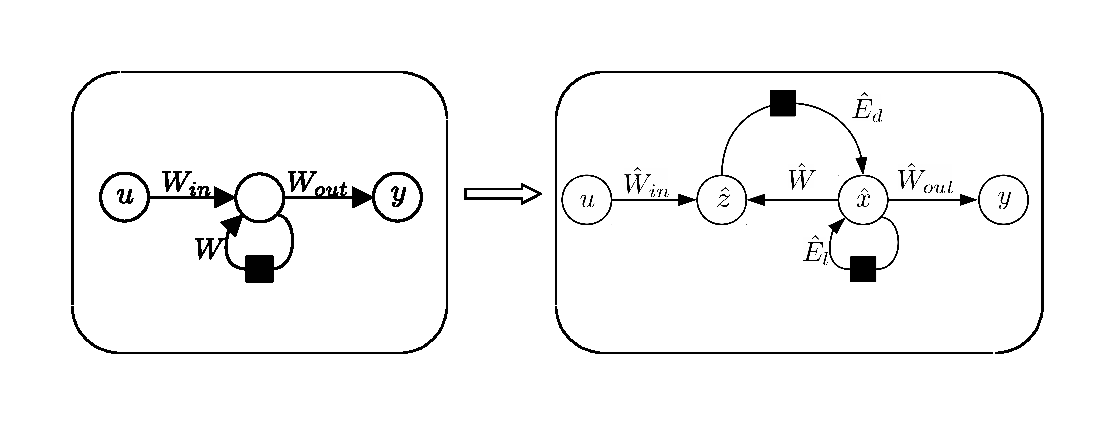
\includegraphics[width=0.7\columnwidth]{ESN_convert.eps}
	\caption{原始网络生成简化网络的示意图}
	\label{fig:esn_convert}
\end{figure}

简化回声状态网络的结构如图~\ref{fig:esn_red} 所示。该网络的深度为四,包括输入层\(u\),输出层\(y\)和两层隐藏层\(\widehat{z},\widehat{x}\)。
其中输入层,输出层和状态层\(\widehat{x}\)保留了原网络相似的结构和映射关系。暂态\(\widehat{z}\)是新引入的结构,其作用在于桥接输入层和状态层,
对流经该层的信息做初步的加工处理。暂态层\(\widehat{z}\)和状态层\(\widehat{x}\)共同组成隐藏层,数据在两层隐藏层之间双向流动,形成一个大的信息回路。
但是两层隐藏层也存在差异,暂态层不存在自循环体,因此传统上意义上不能称为状态,考虑到其也位于数据循环的关键路径,因此称之为暂态。实际上
仅从结构特性而言,暂态层和全连接层有更大的相似度。以上分析了简化网络的结构特性,相较于原网络,既存在保留部分,也添加了新的元素。 

\begin{figure}
	\centering
	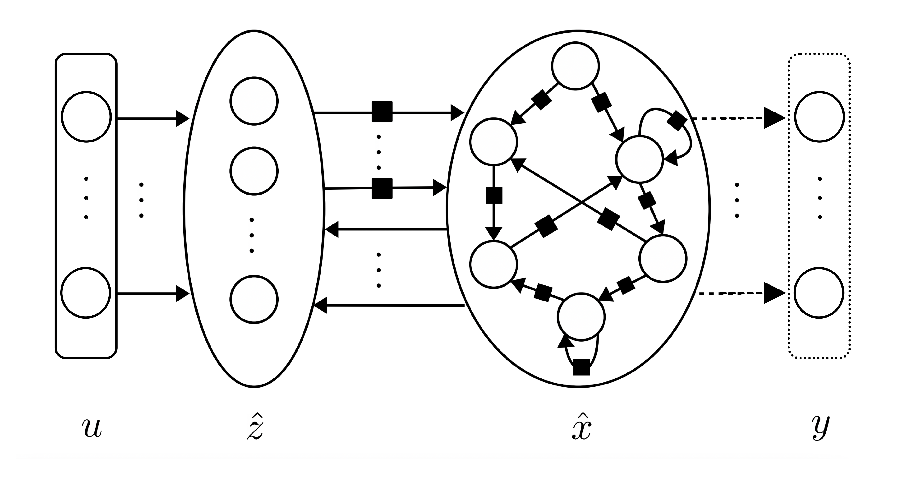
\includegraphics[width=0.7\columnwidth]{ESN_red.eps}
	\caption{简化回声状态网络结构}
	\label{fig:esn_red}
\end{figure}

简化网络的前向传播速度相较原网络会大幅提升,这得益于隐藏层神经元数量的减少。简化网络内部神经元的数量每层\(q\)个,远小于原网络的\(n\)个。
相应的,网络中神经元的连接复杂度也将降低,权重矩阵的参数量将从\(n^2\)变为\(q^2\)。以上神经元数量和权重参数量的压缩将会直观的反映到模型的
计算复杂度上,原网络每个时间步长的前向传播计算复杂度为
\begin{equation}
	\mathcal{O}(n^2 + n n_{in} + n n_{out})
\end{equation}
简化网络的前向传播计算复杂度为
\begin{equation}
	\mathcal{O}(q^2 + q n_{in} + q n_{out})
	\label{eq:computeComplexity}
\end{equation}
在输入输出数量不变的条件下,简化网络的时间复杂度仅由\(q\)决定,和原网络的阶数\(n\)无关。又因为\(q<<n\),所以简化网络前向传播的速度会比原网络快很多。
具体的\(q\)值的选取需根据用户对精度和速度的需求来确定,简化网络的阶数\(q\)越小,模型的计算速度越快;\(q\)越大,模型的精度越高。

\subsection{网络压缩}
前面的叙述介绍了简化回声状态网络和原网络之间在网络结构上的相似性和差异性,解释了简化网络模型预测精度不会显著下降的原因,并从计算复杂度的角度说明了
简化网络在前向传播过程中加速能力的来源,下面本小节将就原网络如何生成简化网络进行简要的说明,模型压缩算法的具体推导请见文献\citing{WangLong:TNNLS'23}。
%介绍高速回声状态网络的生成,算法顺序介绍,or硬件需求倒推
\subsubsection{状态近似}
为了记忆动态系统丰富的时序特性,循环神经网络一般拥有庞大数量的隐藏层神经元,这些神经元互连关系复杂,对信息拥有记忆和遗忘功能,是循环神经
网络最重要的组成部分。对于简单的任务,仅需要少量的神经元便可完成,而复杂的任务则需要更多神经元协同。实际情况下,任务的复杂程度判别具有
相当程度的主观性,隐藏层神经元数量会被保守的设置为远超实际需求的数量,即存在大量的冗余性。本小节针对神经元的冗余性,采用基于投影的状态近似方法进行消除。
状态近似框架:
\begin{equation}
	V_x \widehat{x}_{t} \approx x_{t}
\end{equation}
其中\(V_x \in \mathbb{R}^{n \times q}\)是状态投影矩阵,满足\(V_x^T  V_x = \mathrm{I}\),\(x_{t} \in \mathbb{R}^n\)是状态向量,\(\widehat{x}_t \in \mathbb{R}^q\)是状态近似向量。
状态近似将高维向量\(x_t\)投影到状态空间中,并用状态空间的基向量进行线性表示,其坐标为\(\widehat{x}\)。实际上,由于输出只需要选择性的保留
动态系统过去序列的某些方面信息,而与其他方面无关,系统的动态特征往往有限且集中。这在状态空间上表现为:和任务特性相关的状态只占全部状态的一部分,即
有效状态空间是满状态空间的子空间。按照状态子空间中特征的重要程度划分,有效状态空间又可以分为核心特性空间和外围特征空间。在进行状态投影时,状态向量将首先
被投影到核心特征空间中,在这种状态近似情况下,模型的预测不会偏离真实输出太大;其次,状态将会被投影到外围特征空间,该空间越大,模型就越能捕捉系统微小
的动态特征,模型的输出也就越具有丰富性。状态子空间的选取将会对状态近似后的网络预测效果产生较大的影响,如何构造状态空间以实现较好的近似将在3.1.2.3中介绍。\\
将状态近似框架代入回声状态网络模型~(\ref{eq:esn}) 得到
\begin{equation}
	\begin{split}
		\widehat{x}_{t} & = V_x^T  f(W V_x  \widehat{x}_{t-1} + W_{in}  u_t)	\\
					y_t & = W_{out} V_x  \widehat{x}_t
	\end{split}
\end{equation}
基于投影的状态近似方法生成的简化网络除了隐藏层神经元数量更少以外,还在自循环结构上增加了线性算子。该算子需要在状态激活后
作用于每一个隐藏层神经元,并且运算次数为\(n\),这导致隐藏层的等效神经元数量也为\(n\)。为了获取真正的模型简化,一个直观的想法是将\(V_x^T\)
移动到激活函数内部,形成类似\(V_x^T  W  V_x\)的\(q \times q\)矩阵,这样模型压缩后等效神经元的数量也为\(q\),简化网络前向传播的时间复杂度
也将进一步降低。然而循环神经网络的激活函数通常是非线性的,非线性算子和线性算子的执行顺序是不能更改的,因此此想法无法直接实现。

如果存在矩阵\(P \in \mathbb{R}^{n \times q}\) 能够和非线性运算交换顺序,即矩阵能够穿透激活函数,使得
\begin{equation}
	P^T f(W V_x  \widehat{x}_t + W_{in} u_t) = f(P^T W V_x \widehat{x}_t + P^T W_{in} u_t)	
\end{equation}
那么将会实现回声状态网络真正的简化,其模型大小就完全不受原网络尺寸的影响。如何构造这样一个理想的矩阵,数学上早已给出了充分的研究和证明。
当\(P = [e_1,e_2,...,e_q]\) (\(e \in \mathbb{R}^n\)是只含一个1且其余元素为0的向量),线性运算和非线性运算可以交换顺序。其原理在于矩阵P的
运算只是从n行向量中选出q行,不会改变向量中具体元素的数值,因此不会影响激活函数\(f\)独立的应用到向量的每一个元素。在回声状态网络的数学方程中,
矩阵P的功能是从n个方程中选择q个方程,使得这q个方程的近似解和n个方程的真实解误差最小。关于矩阵P的构造,可以通过离散经验插值方法(Discrete Empirical Interpolation Method,DEIM)
实现,DEIM的完整讨论请参见\citing{DEIM}

\subsubsection{激活函数近似}
投影方法同样也适用于激活函数的近似,\(n\)维的函数\(g(x)\)会被用\(q\)维函数\(\widehat{g}(x)\)替换,这可以减小激活函数的应用次数。但是简单直接的对非线性激活函数
使用投影近似会带来系统不稳定的问题,系统稳定性分析请见文献\citing{WangLong:TNNLS'23}。因此为了得到渐进稳定的简化网络,激活函数将被分为线性部分和非线性部分,
投影近似仅作用于非线性部分。网络隐藏层在系统稳定点0附近的非线性部分可以表示为
\begin{equation}\label{eq:h(x)}
	h(x_t) = f(W x_t + W_{in} u_t) - W x_t
\end{equation}
结合激活函数近似框架
\begin{equation}
	V_h \widehat{h}(x) \approx h(x)
\end{equation}
式中\(V_h \in \mathbb{R}^{n \times q}\)是函数投影矩阵,将选择矩阵P作用于该投影近似框架,得到
\begin{equation}\label{eq:Pselect}
	P_h^T V_h \widehat{h}(x) = P_h^T h(x)
\end{equation}
最后,综合以上理论公式,将得到简化网络的最终形式
\begin{equation}\label{eq:esn_red}
	\begin{split}
		\widehat{x}_t  = &(V_x^T W V_X - \widehat{E}_d P_h^T W V_x)\widehat{x}_{t-1}  \\
					     & + \widehat{E}_{d} f(P_h^T W V_x \widehat{x}_{t-1} + P_h^{T} W_{in} u_{t})	\\
				y_t    = &W_{out} V_x \widehat{x}_t
	\end{split}
\end{equation}
其中,\(\widehat{E}_d = V_x^T V_h (P_h^TV_h)^{-1}\),为进一步简化表达,定义
\begin{equation}
	\begin{split}
		\widehat{E}_l = V_x^T W V_x - \widehat{E}_d P_h^T W V_x,	\qquad &\widehat{W} = P_h^T W V_x,		\\
		\widehat{W}_{in} = P_h^T W_{in},							\qquad &\widehat{W}_{out} = W_{out}V_x
	\end{split}
\end{equation}
将以上表达代入~(\ref{eq:esn_red}) 即可得到简化网络的模型~(\ref{eq:redesn}) 。

\subsubsection{状态采样和函数采样}
以上从数学的角度展示了回声状态网络如何一步一步的从原网络生成简化网络的过程,其中所使用的投影近似框架和DEIM是模型压缩中常见的方法,也适用于其他神经网络模型的压缩,
目前已经在LSTM,GRU等循环神经网络模型上检验过压缩效果。为使模型压缩的理论具有连续性,上述推导过程都是假设投影矩阵\(V_x,V_h\)以及选择矩阵\(P\)存在的基础上进行,
省略了如何构造这些矩阵的过程。然而,从工程的角度,如何构造这些矩阵并由这些矩阵生成简化网络的权重是更受关注的。本小节将通过状态采样和函数采样
的方法解决这一遗留问题。

状态采样是指在回声状态网络前向传播的过程中,采集一段不同时间点下的原始系统状态样本\(\{x_1,x_2,...,x_{n_s}\}\)形成状态空间。由于回声状态网络的隐藏层权重不可训练,
采样的状态空间也就和训练过程无关,其只决定于系统的初始化特性和输入序列特征。理论上,样本越丰富,状态空间就越能还原动力系统的真实特性。

同理,函数采样是指采样原网络前向传播过程中不同时刻的激活函数样本,实际上是激活函数近似框架中的非线性部分,如式~(\ref{eq:h(x)})所示。函数采样
将得到激活函数空间\(\{h_1,h_2,...,h_{n_s}\}\)。

在完成状态采样和激活函数采样后,将会对采样空间进行奇异值分解~(SVD) 以寻找可以作为投影面的一组标准正交基,如下所示:
\begin{equation}
	\begin{split}
		V_x \Sigma_x U_x^T \ \xleftarrow{SVD} \ X;	\qquad	H \ \xrightarrow{SVD} \ V_h \Sigma_h U_h^T 	
	\end{split}
\end{equation}
其中\(X = [x_1,x_2,...,x_{ns}] \in \mathbb{R}^{n \times n_s} \),\(V_x \in \mathbb{R}^{n \times n_s},U_x \in \mathbb{R}^{n_s \times n_s}\),\(\Sigma_x \in \mathbb{R}^{n_s \times n_s}\)
是状态空间及其分解的子空间;\(H = [h_1,h_2,...,h_{ns}] \in \mathbb{R}^{n \times n_s} \),\(V_h \in \mathbb{R}^{n \times n_s},U_h \in \mathbb{R}^{n_s \times n_s}\),\(\Sigma_h \in \mathbb{R}^{n_s \times n_s}\)
是激活函数空间和其分解的子空间。分解后的矩阵中,奇异值矩阵\(\Sigma\)和原矩阵是一一对应关系,左奇异矩阵和右奇异矩阵互为依赖,其作为一个整体和原矩阵保持对应关系。
由于这种对应关系的存在,以及其标准正交特性,奇异矩阵可以作为原空间的近似并且可以当作投影矩阵。本文将左奇异矩阵\(V\)作为投影矩阵。

为了减少与任务关联度低的特征在特征空间中所占的比例,这里选择保留\(V\)的前\(q\)列作为投影矩阵。
\begin{equation}
	V_x \ \leftarrow \ V_x[:,1:q];	\qquad V_h \ \leftarrow \ V_h[:,1:q]
\end{equation}
由于\(V\)的前q列对应\(\Sigma\)中最大的q个奇异值,所以此截断方法保留了原始矩阵最重要的信息,在特征空间中反映为:选取最重要的q个特征向量组成新的子空间,
尽管该特征子空间的维度远小于原始特征空间,但是高维特征却能以较小的精度损失投影到该子空间。关于q值的选取,往往不存在一个最优选项,需要根据
应用场景对精度的实际需求进行确定,q值越大,损失的信息越小,精度越高。

以上基于状态采样和函数采样获得了投影矩阵\(V_x,V_h\),为了获取简化网络权重矩阵所需要的全部要素,还需要确定选择矩阵\(P_h\)。P首次出现在(\ref{eq:Pselect}),
其功能是从n个非线性方程中选出q个方程进行求解。由于每个方程有q个变量,并且非线性方程对应的函数是单调函数,因此求解出这q个变量实际所需的方程数也是q,但是
激活函数具有饱和特性,存在较大数值差异的自变量对应“相同”函数值的情况,因此需要找出这些方程,并选出其中一个方程作为代表,使得方程组的解和原方程组的
真实解误差最小。DEIM是一种基于贪婪思想从n个非线性方程中选择q个有精确“近似”方程的方法,该方法一个接一个的选出使得解向量的误差最小的方程组,并最终选出q个符合要求的方程。
这里不再详细展示DEIM的推导过程,只展示本文用到的算法,如算法~\ref{alg:deim} 所示。
\subsection{压缩算法的评估与分析}
前面的小节展示了回声状态网络的简化网络结构,以及如何从原网络一步一步生成这样一个简化网络。本小节将对简化网络的实际运行效果进行评估,以证明
压缩算法的有效性和可行性,本小节的验证实验在Intel i5-8500 CPU计算平台上进行。

首先,模型的压缩需要在保证模型的基本功能正常的前提下进行,脱离任务实际需求,仅考虑压缩率的模型压缩算法是往往无效的。图~\ref{fig:accuracy} 所示为简化网络
在NARMA10系统上的精度表现,其中原网络的模型大小为500阶,其模型预测值能较好的贴近系统真实值,尤其是在系统真实输出剧烈变化的位置,原网络能捕捉这种动态信息,
但是相对于其他变化平缓的区段,误差显得更大。简化网络的模型大小为80阶,远小于原网络的尺寸,但是其模型预测精度并没有大幅下降,图中显示简化网络
的预测值和系统真实输出也能保持较好的贴合度。在系统输出变化时,简化网络的输出会保持变化方向的一致性,尽管在数值上存在差异。由于简化网络是由原网络生成的,没有
在数据集上训练,因此原网络的精度是决定简化网络预测效果的直接因素,图中显示,简化网络的预测值和原网络的预测值在多数情况下能保持一致,除了个别位置波动较大。
误差是不可避免的,本文所使用的模型压缩算法能在可接受的误差范围内实现模型尺寸的压缩,是一种可行且有效的循环神经网络压缩方法。
\begin{figure}
	\centering
	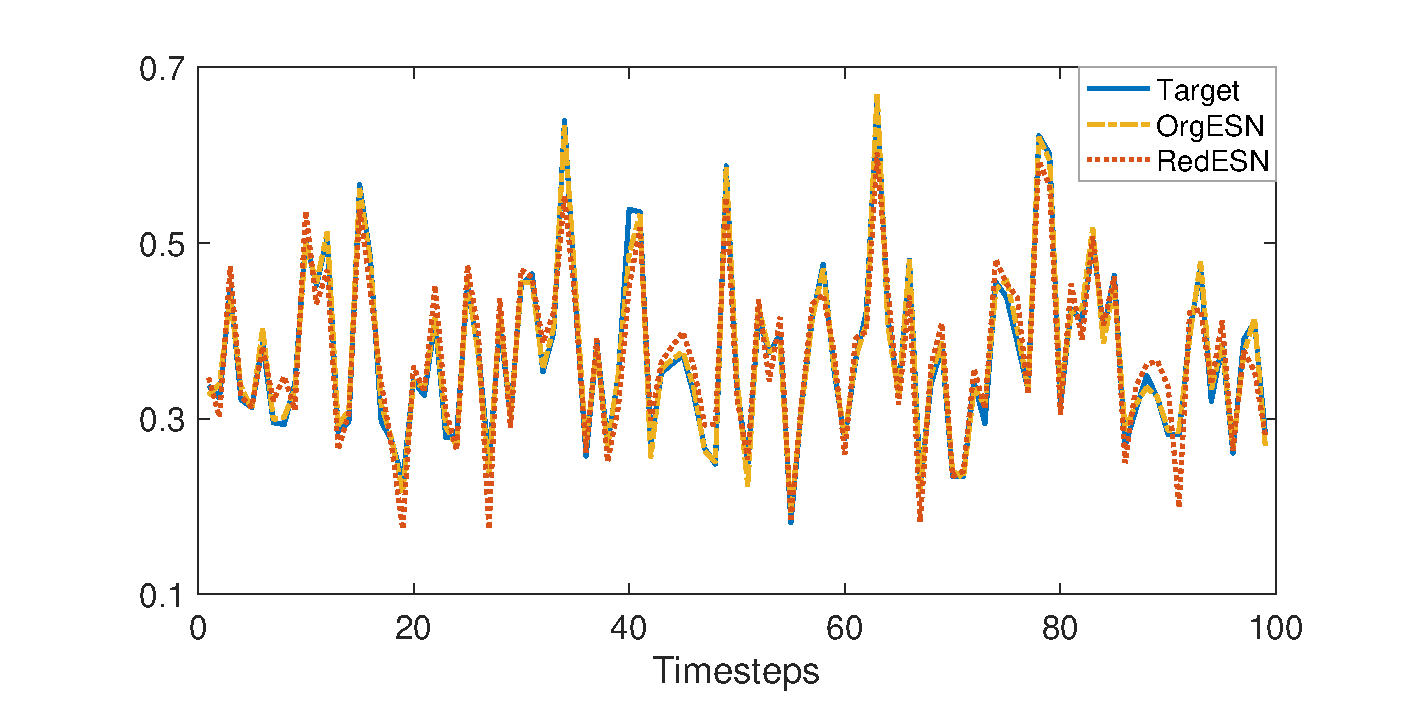
\includegraphics[width=1.0\columnwidth]{exp/500&80_all.eps}
	\caption{ESN简化网络和原网络在NARMA10系统上的精度效果,原网络(OrgESN)为500阶,简化网络(RedESN)为80阶}
	\label{fig:accuracy}
\end{figure}

其次,模型压缩算法的目的是降低模型计算的时空复杂度,实现神经网络前向传播过程的加速。表~\ref{tab:accuracy} 所示为模型参数量,预测精度和速度。其中500表示原网络的尺寸,
其余尺寸代表不同阶数的简化网络。从参数量的角度,简化网络的参数量少于原网络,且压缩力度越大,参数量减少越明显。参数量的多少直接决定着模型
的存储开销,显然简化网络能有效节约存储空间。从推理速度的角度,简化网络的完成全部序列的推理所需要的时间明显小于原始网络,这是因为简化网络的的计算量更小。
最后从模型预测误差的角度,简化网络的精度损失更大,但是都没有超出可接受范围,并且随着模型尺寸的增加,精度也在上升。随着简化网络尺寸的增大,以损失预测精度而产生的模型压缩加速收益
逐渐降低,并最终趋于0,因此在应用过程中需要根据实际情况选择合适的简化网络尺寸。

综上所述,压缩算法在保证模型预测精度不显著下降的情况下,大幅的降低模型参数量,减轻了硬件计算平台存储和计算的压力,并最终达成了对模型前向传播过程加速的目的。

\begin{center}
\begin{table}
	\caption{不同尺寸模型的参数量,推理速度和精度}
	\begin{tabular}{cccccccc}
		\toprule
		 Size			&				500		&	10		&	20		&	30		&	40		&	60		&	80		\\	\midrule
		 Parameters		&				26k		&	0.3k	&	1.2k	&	2.8k	&	4.9k	&	11k		&	19k	 	\\	
		 Times (s)		&				0.48	&	0.17	&	0.17	&	0.18	&	0.18	&	0.19	&	0.21	\\	
		 MSE\(\times 10^{-3}\)&		0.13	&	4.9		&	1.7		&	1.7		&	1.6		&	1.6		&	1.3		\\
	\bottomrule
	\label{tab:accuracy}
	\end{tabular}
\end{table}
\end{center}

\section{系统整体架构设计}
在前叙压缩算法的工作基础上,本章接下来将对算法特性进行深入分析,并结合应用场景,提出一套针对循环神经网络前向传播过程的加速系统,该系统能根据用户和实际
环境的性能需求匹配相应的网络模型预测精度和速度,做到既不会性能过剩,也不会性能不足。然后,针对系统的具体实现,本章将从软硬件的角度考量系统各个组成部分实现的成本和收益,
并进行软硬件划分与协同,以最大化系统的实现效率。最后,本章将选用FPGA作为硬件计算平台,实现本文所设计的循环神经网络加速系统。
\subsection{前向传播及压缩流程}
本文采用基于投影的压缩算法进行模型压缩,压缩后简化网络的模型尺寸不受原网络的影响,并且该尺寸可以进行调节,当简化网络的尺寸设定为较大的
值时,可以实现较高的预测精度;当简化网络的尺寸设定为较小值时,模型前向传播的速度会加快。这种网络尺寸可调的特性赋予了神经网络在算法层面的弹性计算能力。
同时,随着模型尺寸的伸缩变化,网络的预测效果将会在速度或精度方面得到增强,从而满足用户动态调节模型预测精度和速度的需求。通常情况,模型压缩算法都可以控制
压缩的尺度,并且产生不同的模型预测效果,例如剪枝技术可以调节模型的稀疏度,量化方法可以调节数据字长等。相较而言,本文的模型尺寸调节是指改变网络的结构,
与上述方法相互独立,并且由于其完善数学推导,在相同精度损失的条件下,往往能获得更高的模型压缩率。以上是简化网络前向传播过程的分析,其具有
模型尺寸可调的特点,能满足应用场景的弹性性能需求。

状态采样和激活函数采样形成的样本集是生成简化网络所需要的全部数据来源,采样过程是伴随原网络的前向传播过程同时发生,而与反向传播无关,因此压缩算法所
需的数据和模型训练集无关,更具体的,其仅决定于原网络的隐藏层特性和任务的输入序列特性。这种无数据集的特性赋予了压缩算法使用场景极大的自由度,
一些特殊场景如数据集获取成本大的场景,训练方法保密场景等往往不公布数据集,仅提供可前向传播的模型,传统的模型压缩算法将难以为继,而本文的压缩算法
依然可以发挥功效。以上是本文所采用算法的第二大特性---无需数据集,这使得算法的应用场景被拓宽。

投影方法包含矩阵分解和DEIM两大过程,相比于其他神经网络压缩算法需要反复迭代和微调等复杂流程,本文压缩算法的实现成本小。实际上,有关线性代数
在硬件上的加速与优化已经存在大量的成果,如BLAS,LAPACK,NumPy,以及本文所使用的针对嵌入式设备而开发的函数库Eigen。
丰富的开发工具和优化过的实现方案使得本文的压缩算法的实现成本进一步降低,甚至可以在资源有限的边缘的边缘设备上实现。以上是本文所采用算法的第三大特性
---压缩算法实现成本低,这使得网络的压缩过程可以在资源有限的设备上独立完成。
\begin{figure}
	\centering
	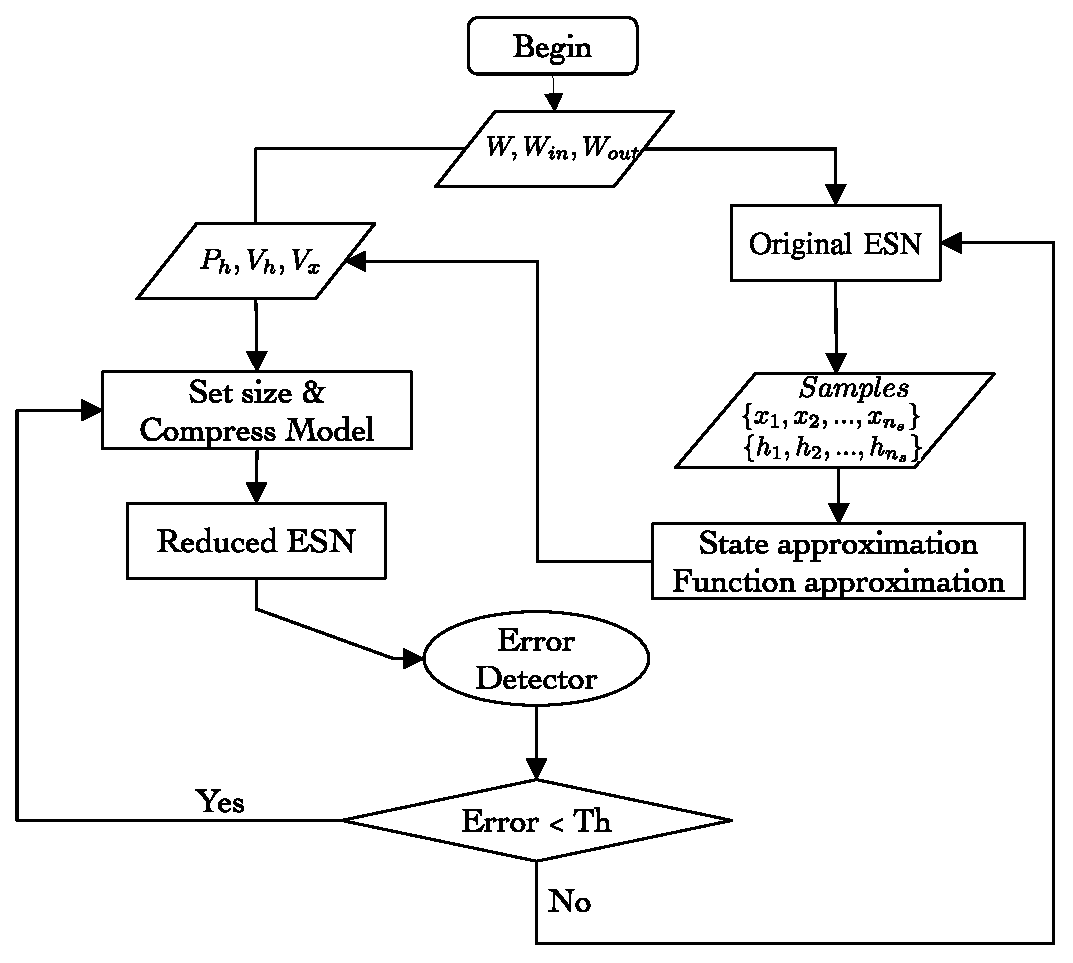
\includegraphics[width=0.6\columnwidth]{exp/Flowchart_diagram.eps}
	\caption{循环神经网络前向传播加速和压缩流程图}
	\label{fig:flowchart}
\end{figure}

基于以上循环神经网络前向传播过程和压缩算法特性的深入分析,接下来,本文将提出符合算法特性,并且考虑实际应用场景需求和约束的循环神经网络加速系统。
该系统能根据用户和环境对模型预测精度和速度的实际需求动态地调节网络模型的尺寸,使得模型预测精度或速度恰好达到用户的要求。同时系统的设计考虑了硬件计算平台的独立性,通过闭环的
系统流程实现了系统在边缘设备的完整运行。循环神经网络前向传播与加速的系统流程如图~\ref{fig:flowchart} 所示。首先需要向加速系统预存初始化参数,
包括循环神经网络的权重参数(\(W,W_{in},W_{out}\))和模型压缩过程所需的投影矩阵(\(V_x,V_h\)) 及选择矩阵(\(P_h\)),然后系统会根据用户设定的模型尺寸生成
相应尺寸的简化网络权重参数,该过程只需要进行简单的矩阵乘法就可实现。最后,系统会执行简化网络的前向传播算法。当系统运行在普通状态环境中,并且误差较小时,
用户可以调整投影空间的大小并基于此直接生成简化网络模型参数,实现系统预测速度的调整;当系统运行在异常状态环境时,即系统的误差较大且无法通过提高简化网络尺寸的方式进行降低时,
说明简化网络在模型压缩过程中丢失了这一段序列的
的动态信息,因此需要结合该段序列重新生成简化网络的权重参数。此时,系统将运行原始网络模型并对该段序列输入所产生的状态进行采样,形成状态样本集和
激活函数样本集,最后在状态近似和激活近似的框架下,样本集将生成\(V_x,V_h,P_h\)等压缩过程需要的全部信息。以上运行原网络并采样实现了系统和环境的数据交互,
并最终补偿了简化网络的预测精度。
\subsection{软硬件功能划分}
在确定算法特性,应用场景需求和系统运行流程后,本小节将进一步确定系统的具体实现方式。通常情况,电子系统的实现包括软件和硬件两种方式。
软件实现是指采用C/C++等高级程序语言描述系统的行为,代码最终以串行执行的方式运行在通用处理器上,具有实现成本低,灵活性强等优势,擅长处理分支判断等
流程控制类任务,其劣势在于并行化程度低,计算周期长。硬件实现克服了软件的劣势,通过对资源进行空间复用,硬件实现可以轻易获得很高的并行度,从而实现
大规模批量化的处理数据。同时,相较软件执行过程,硬件实现通常是为具体应用量身定制,无需繁杂的编码解码过程,从而节省了能量消耗,具有高性能计算的特点。
然而,硬件实现方式也存在明显的劣势,包括灵活性差,资源开销大以及开发周期长等。因此,综合软硬件实现的优势,本文采用软硬件协同的方式对系统进行
设计实现。

系统功能的软硬件划分是否合理直接决定这系统能否高效运转。本文系统的功能划分如表~\ref{tab:soft&hard} 所示。首先,根据任务的目的对系统进行初步的划分,
系统被分解为推理部分和压缩部分两个主要部分。其中推理任务需要执行包括原始网络和简化网络两种不同结构模型的前向传播过程,而对简化网络前向传播过程进行加速是
本文系统设计的首要目标,并且其面临着低延迟,低功耗的约束,因此简化网络的前向传播将优先采用硬件实现的方式。从算法特性的角度,模型包含大量可并行计算
的单元,主要体现在矩阵向量乘法中,这能充分发挥硬件的优势。在简化网络实现方式确定的基础上,由于原始网络结构的基本组成单元和简化网络相同,因此针对结构上共性,
可以考虑共用一套硬件模块,对于少量较大差异的部分则单独设计硬件单元,但是额外的硬件开销应当尽量的减少,并且由于运行原始网络的目的不是用于实际的模型预测,而仅
用于采样压缩算法所需要的数据,因此节约硬件资源是首要设计目标。以上是对推理过程实现方式的分析,考虑到系统设计目标及实现的成本,网络的前向传播过程将采用专用
硬件架构进行实现。模型压缩任务可以更具体的划分为矩阵奇异值分解(SVD),离散经验插值(DEIM)和简化网络生成。尽管这些功能模块都是将矩阵
作为基本操作对象,但是算法的复杂度高,并且从执行频次的角度,模型压缩的需求是存在的但却不会频繁地请求。因此,本文压缩过程的所有任务都将采用
软件的方式实现。

\begin{center}
\begin{table}
\caption{系统功能模块与软硬件划分}
\renewcommand\arraystretch{1.3} 
\setlength{\tabcolsep}{5mm}{
\begin{tabular}{|c|c|c|}
\hline
\multirow{4}{*}{推理过程}	&	简化网络前向传播		&	\multirow{4}{*}{硬件实现}		\\	\cline{2-2}
							&	原始网络前向传播		&									\\	\cline{2-2}
							&	状态采样				&									\\	\cline{2-2}
							&	激活函数采样			&									\\
					\hline \hline	
\multirow{3}{*}{压缩过程}	&	奇异值分解(SVD)		&	\multirow{3}{*}{软件实现}		\\	\cline{2-2}
							&	离散经验插值(DEIM)	&									\\	\cline{2-2}
							&	简化网络生成			&									\\	
					\hline
\end{tabular}
}
\label{tab:soft&hard}
\end{table}
\end{center}

\vspace{-3em}

以上分析了软硬件实现方式的优势和劣势,并对系统功能进行了划分,综合考虑实现成本,硬件资源开销,系统目标及任务需求等方面因素,本小节将系统各功能
模块映射到合适的实现方式上,初步完成了循环神经网络前向传播与加速系统的设计,本文将在后续章节详细的介绍具体实现细节。
\subsection{系统整体架构}
在完成系统功能模块和软硬件实现方式的匹配后,系统的整体架构也就自然而然的浮现出来。图~\ref{fig:sysArch} 所示为本文系统的SoC实现架构。
从实现方式的角度,该架构主要由三部分构成:软件部分,硬件部分以及软硬件接口界面。对应的,其硬件基础分别为:CPU,加速器和AXI总线。从硬件模块功能的
角度,系统架构可以分为处理器模块(CPU和加速器),存储模块(片上存储和片外存储)以及互联模块。以上从不同的角度对系统进行解构,系统的全景图被清晰的展现出来,
实际上系统的高效运转需要有机的结合各个组成部分。

系统架构中的各个模块具有不同的特性,并分别承担符合其工作模式的一部分系统功能。其中CPU模块负责运行软件端代码,通过控制总线对硬件加速器进行配置和控制,
通过数据总线向加速器载入参数和输入数据,并最终将硬件执行的结果返回到软件端。加速器部分主要完成系统划分给硬件实现的功能,包括循环神经网络的
前向传播过程以及数据采样。加速器的设计采用冯诺伊曼的存算分离结构,其由控制单元,运算单元和存储单元组成。存储单元一方面是作为缓存与片外存储
交换数据,另一方面作为寄存器用于暂存计算单元产生的中间数据,其存在的意义是减少计算单元访问片外存储的频率,利用其高速的特性降低数据移动所带来的延迟。
控制单元通过对计算单元和存储单元进行控制完成任务的具体功能,同时根据系统设计目标,本文的控制器需要具有可配置的特性,在接收CPU传输的配置信息后
需要控制加速器实现不同的功能,包括切换网络结构和改变模型尺寸。 计算单元由矩阵-向量乘法(MVM)模块和激活函数模块构成,由于循环神经网络存在大量的乘加运算
操作,这使得计算单元面临着较重的任务负载,并且耗时较长。通常情况下,计算单元和存储单元需要进行高速化设计,采用并行化和流水线化技术进行优化,
这也是神经网络加速器加速能力的来源。
\begin{figure}
	\centering
	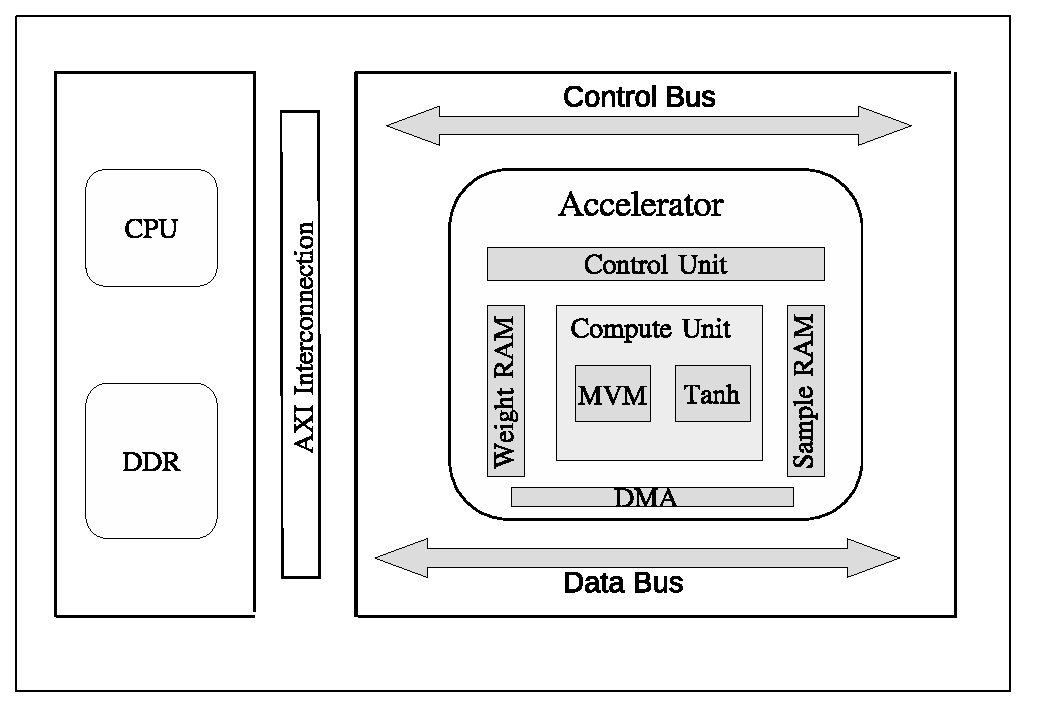
\includegraphics[width=0.8\columnwidth]{exp/fig_systemArch2.eps}
	\caption{系统整体架构图}
	\label{fig:sysArch}
\end{figure}

\section{压缩过程的软件实现}
前一节系统的划分确定了软件端需要实现的功能,本小节将对这些功能逐一进行实现,包括功能的细化,软件架构的定义以及算法的开发。在功能方面,软件端总体上可
划分为两大部分。其一是压缩过程的软件实现,该过程需要用到线性代数相关运算,特别是矩阵分解和线性方程求解。通常情况下,矩阵相关的任务可以
采用硬件实现,但时考虑到实现的成本和收益,本文对压缩过程的全部子过程均使用软件的方式实现。压缩过程首先需要从硬件加速器端的存储
单元读取状态样本和激活函数样本,然后对样本集进行分解并选取样本空间的一部分特征子空间作为投影空间。为了进一步获得更简化的网络模型,采用离散经验
插值的方法改变线性运算和非线性运算的顺序,使得矩阵乘法能够穿透激活函数进而与函数内部的常量矩阵相乘,获得更小的计算复杂度。最后,根据以上
计算过程所获得的投影矩阵和选择矩阵,将原始网络的权重参数转化为简化网络的权重矩阵,并最终完成模型的压缩过程。为了便于软件实现,算法~\ref{alg:GenPUV},\ref{alg:deim}和~\ref{alg:GenESN}分别
就生成投影矩阵和选择矩阵,离散经验插值以及生成简化网络权重参数等压缩过程关键步骤作出详细的描述。在功能上,这些算法层层递进,既相互独立以完成各自的功能,
又相互依赖以实现系统级的功能。算法的分层所带来的好处是系统功能更加细化且明确,例如算法~\ref{alg:GenESN} 是压缩过程中最顶层的描述,其输入信息为
投影矩阵和选择矩阵等关键压缩信息以及原始网络的权重参数信息。关于投影矩阵和选择矩阵的获取,一方面可以通过执行算法~\ref{alg:GenPUV} 和~\ref{alg:deim} 
获取,另一方面可以通过预存关键矩阵进行实现,这种算法的分层描述极大的拓宽了系统功能实现的自由度。
%算法\ref{alg:Gen_ESN}
%展示了压缩过程的算法描述,算法\ref{alg:deim}是补充说明。DEIM算法被单独列出,一方面是因为其功能的独立性,另一方面是因为算法\ref{alg:Gen_ESN}描述
%的简洁与连贯。算法\ref{alg:Gen_ESN}总体上可以划分为两部分,分别是关键矩阵的生成和简化网络的生成。这两部分存在数据依赖关系,但是功能又相互独立。
%为了使功能界限更加明显,可以通过预存关键矩阵的方法实现这两部分的分离。


算法定义了软件程序的边界,抽象程度越高的算法往往实现系统层级的功能并和应用高度绑定,如算法\ref{alg:GenESN}实现了系统功能中压缩过程,抽象层级较低的算法往往具有通用的功能,
如算法\ref{alg:deim}。算法描述的最底层应当是工具所能提供的不可分化的功能单元,如SVD,Solve等函数。Eigen是专为嵌入式软件设计的线性代数库,
提供了压缩算法最基本的实现单元。本文软件实现正是基于此函数库从而构建模型压缩的功能,程序的层级也如算法的抽象层级一般,分层实现。

\begin{algorithm}
\setstretch{1.2}
 \SetKwInOut{Input}{Input}\SetKwInOut{Output}{Output}
 \Input{samples\(\{x_1,x_2,...,x_{n_s}\}\) and \(\{h_1,h_2,...,h_{n_s}\}\), \\
	    Pre- reduced order \(n_q\)}
 \Output{Projection matrix $V_x,V_h$,Selsection Matrix $P_h$}
\emph{$\triangleright$\ Obtian the state approximation matrix \(V_x\)}\;
$ X \leftarrow [x_1,x_2,...,x_{n_s}]$	\;
$ V_x,\Sigma_x,U_x \leftarrow SVD(X)$	\;
$ V_x \leftarrow V_x[:,1:n_q]$	\;

\emph{$\triangleright$\ Obtian the function approximation matrix \(P_h\) and \(P_h\)}\;
$ H \leftarrow [h_1,h_2,...h_{n_s}] $	\;
$ V_h,\Sigma_h,U_h \leftarrow SVD(H)$	\;
$ V_h \leftarrow V_h[:,1:n_q]$	\;
$ P_h  \leftarrow DEIM(V_h)$	\qquad \emph{$\triangleright$ DEIM process in Algorithm 2}\;

 \caption{Generate Porjection matrix and Selection matrix}
 \label{alg:GenPUV}
\end{algorithm}
\begin{algorithm}
\setstretch{1.2}
 \SetKwInOut{Input}{Input}\SetKwInOut{Output}{Output}
 \Input{$V_h \in \mathbb{R}^{n \times n_s}$ and Pre-reduced order \(n_q\)}
 \Output{$P_h \in \mathbb{R}^{n \times q}$}
$[u_1,u_2,...,u_q] \leftarrow V_h[:,1:n_q]$	\;
$\rho$ = maxIndex$(|u_1|)$							\;
$P = [e_{\rho}]$, \quad $U = [u_1]$			\;
for $\ell = 2$ \ to \(n_q\) 							\;
\qquad	Solve$(P^T U c) = P^T u_{\ell}$ \ for c	\;
\qquad	$r = u_{\ell} -Uc$						\;
\qquad	$\rho =$ \ maxIndex$(|r|)$						\;
\qquad	$U \leftarrow [U,u_{\ell}], P \leftarrow [P,e_{\rho}]$		\;
end for	
 \caption{DEIM}
 \label{alg:deim}
\end{algorithm}



\begin{algorithm}
\setstretch{1.2}
 \SetKwInOut{Input}{Input}\SetKwInOut{Output}{Output}
 \Input{key matrix $P_h,V_h,V_x \in \mathbb{R}^{n \times n_q}$,		\\
	 	Original ESN matrices $W,W_{in},W_{out}$,	\\
	 	reduced order q (q<\(n_q\)).}
 \Output{ReducedESN weight matrices $\widehat{E}_d, \widehat{E}_l, \widehat{W}, \widehat{W}_{in}, \widehat{W}_{out}$}

 $V_x \leftarrow V_x[:,1:q]$	\;
 $V_h \leftarrow V_h[:,1:q]$	\;
 $P_h \leftarrow p_h[:,1:q]$	\;
 \emph{$\triangleright$\ Generate RedecedESN matrices	}	\;
$\widehat{E}_d \leftarrow V_x^T V_h (P_h^T V_h)^{-1}$	\;
$\widehat{E}_l \leftarrow V_x^T W V_x - \widehat{E}_d P_h^T W V_x$	\;
$\widehat{W} \leftarrow P_hT W V_x$	\;
$\widehat{W}_{in} \leftarrow P_h^T W_{in}$	\;
$\widehat{W}_{out} \leftarrow W_{out}V_x$	\;

 \caption{Generate ReducedESN from OriginalESN}
 \label{alg:GenESN}
\end{algorithm}

软件实现的第二大功能是流程管理和硬件配置等控制类功能。该部分软件程序需要接收外部环境的输入信息,包括简化网络模型尺寸切换的指令,运行原始网络并进行采样
的指令以及简化网络生成指令等。在接收到指令后,软件需要对系统的流程作出调整。例如当系统监测到模型的预测精度降低时,需要将简化网络的模型尺寸
重新设定为较大的阶数,在完成模型压缩后需要进一步判断误差是否降低,以及是否需要运行原网络以进行精度补偿。系统对硬件的控制也在软件端实现,
具体功能包括配置网络结构以完成原始网络和简化网络的切换,配置简化网络的模型尺寸以实现应用环境对系统精度和速度的要求,启动网络的前向传播并
接收硬件加速器计算的结果。

\section{前向传播过程的硬件分析与设计}
\subsection{前向传播过程分析}
循环神经网络的前向传播过程是系统需要实现的最主要功能,该过程需要根据输入序列预测动态系统的行为。系统的预测能力一方面体现为预测精度,另一方面
表现为预测速度。相比于传统的单方面追求速度或资源消耗的神经网络硬件实现,本文的设计还需要考虑预测精度的因素。由于系统的预测精度和速度是一组
难以调和的矛盾,不可同时兼得,所以本文在神经网络加速器的设计上赋予了系统精度和速度灵活的可调节空间,具体的预测能力需求则交由用户和环境决定。
为了实现预测精度和速度可调这一系统功能,本文的神经神经网络加速器需要具备以下能力:

1. 本文的神经网络加速器需要拥有调节网络模型尺寸的能力。当加速器运行小尺寸网络时,系统将获得高预测速度;当加速器运行大尺寸网络时,系统将获得高预测精度。

2. 为了能准确的生成不同尺寸的网络模型参数,本文的神经网络加速器拥有采样数据的能力。采样数据是指采样原始网络前向传播过程中的状态数据和激活函数数据。

3. 为了配合数据采样功能,本文的神经网络加速器需要具备切换不同网络模型的能力。当加速器需要调节简化网络的模型尺寸时,其需要先切换到原始网络模型
并运行一段时间,以采用足够的数据供压缩算法使用。 

%1需要实现原始网络,高速网络两个网络结构。
%2压缩网络结构尺寸可调节。
%3模型压缩过程。
\subsection{加速器整体架构}
前一小节从算法需求的角度为加速器提供了设计目标,本小节结合算法特性和硬件约束将设计目标转化为定制化专用硬件架构。循环神经网络前向传播算法的
基本运算单元包括矩阵向量乘法和非线性激活函数,通过组合这些基本单元,网络拥有了复杂的分层结构。在硬件实现层面,基本结构的不同组合方式呈现
出不同的资源,速度和功耗等硬件特性,即代表着不同的加速器架构。两种比较极端的设计方案分别是网络折叠为基本结构和网络全部展开,这两种
方案代表着极致的节约资源和追求速度。在普通应用场景中通常需要在综合考虑两种方案的优势,对于资源消耗大的硬件单元则应该尽量采取折叠的设计方案,
而对于决定系统速度的关键部分则应该使用展开的设计方案。在硬件资源的约束和网络推理速度的要求下,本文的加速器采用了结构级模块并行和
分时复用的设计方案,既能降低加速器辅助功能的资源开销,又能实现网络前向传播的加速。
\begin{figure}
	\centering
	\includegraphics[width=0.9\columnwidth]{exp/fig_accArch.eps}
	\caption{加速器整体架构。由运算单元,存储单元和控制单元组成}
	\label{fig:accArch}
\end{figure}

图~\ref{fig:accArch} 是本文加速器的整体架构,其采用了冯诺伊曼的存算分离的设计方法,主要部件包括存储单元,计算单元和控制单元。存储单元由权重存储单元(Weight RAM)
和状态存储单元(Samples RAM)组成,在网络前向传播过程中完成模型权重缓存和采样数据存储的功能。运算单元由矩阵向量乘法模块(MVM),激活函数模块(Tanh)和乘累加模块(MAC)
构成,主要承担着网络前向传播过程的数据计算功能。控制单元以状态机的形式实现,通过使能不同的数据路径,加速器能够运行不同的网络模型,同时控制单元能根据软件端的配置信息实现
调节简化网络模型尺寸的功能。

本文加速器架构的设计兼顾了高速和低资源消耗的设计要求。对于延迟敏感的功能如简化网络的前向传播,本文采用了网络展开和模块并行的设计方式,在加速器的架构设计
中具体体现在使用了两个矩阵向量乘法模块,其分别代表着简化网络两层隐藏层的运算。由于两层隐藏层存在数据依赖,无法完成真正意义的并行加速,为了获得近似并行
的计算效果,加速器的设计采用了流水线的方式,两个隐藏层的运算在时间上实现了重叠。对于系统低频使用的功能如原始网络的前向传播与状态采样,本文采用了模块共享
的分时复用设计方式,通过共享简化网络模块中的矩阵向量乘法单元和激活函数单元,加速器实现了原始网络的前向传播功能。相比于简化网络,基于模块
共享方法设计的原始网络结构在资源消耗方面,仅需要增加多路复用器和少量的控制逻辑,这有效的降低了硬件资源的消耗。


%介绍图,模块的划分,复用性体现在哪里,加速体现在哪里
%硬件模块划分与复用性分析

\subsection{计算架构设计}
神经网络加速器是以计算单元为核心的专用硬件结构,而计算单元的本质又是乘法器,加法器以及其他运算部件的组合,如何高效的利用这些基本部件实现更高层级的功能
是计算架构设计面临的最重要的问题。根据前向传播过程分析和系统整体架构设计,计算单元所需要完成功能包括矩阵向量乘法和激活函数,其中激活函数的设计将在后面的
小节中详细讨论,所以本小节将就高效的实现矩阵向量乘法展开详细的说明。

由于本文系统可以调节网络尺寸并以不同尺寸的网络模型进行前向传播,这就要求矩阵向量乘法的尺寸具有伸缩调节的能力,但是一种硬件结构往往只能对应
一种矩阵向量维度,不具备灵活调节的功能。因此如何实现多尺寸矩阵向量乘法是计算单元首先要考虑的问题。解决该问题需要从算法特性层面将矩阵向量乘法
抽象为更基本运算的组合,通过对组合方式进行配置以实现不同的运算功能。

矩阵向量乘法的数学表达为式~(\ref{eq:MVM_element}) 所示,向量\(c\)中的每个元素的生成需要将矩阵\(A\)中对应行与向量\(b\)进行元素乘累加操作。
因此抽象出来的基本运算单元是一个乘累加单元,通过不断的调用该单元,最终实现了矩阵向量乘法,并且通过调节调用次数,可以实现任意维度的矩阵向量乘法。
但是这样的设计没有并行空间,也即无法完成加速计算的目的。
\begin{equation}
	A_{nn}b_n = 
	\begin{pmatrix}
		a_{11} & a_{12} & \cdots & a_{1n} \\
  		a_{21} & a_{22} & \cdots & a_{2n} \\
  		\vdots  & \vdots  & \ddots & \vdots  \\
  		a_{n1} & a_{n2} & \cdots & a_{nn} 
 \end{pmatrix}
	\begin{pmatrix}
        b_{1}	\\ 
        b_{2}	\\
		\vdots	\\ 
        b_{n} 
	\end{pmatrix}
  =
	\begin{pmatrix}
        c_{1}	\\ 
        c_{2}	\\
		\vdots	\\ 
        c_{n}  
     \end{pmatrix}
\label{eq:MVM_element}
\end{equation}
$$c_{i}= a_{i1} b_{1} + a_{i2} b_{2} +\cdots+ a_{in}b_{n} = \sum_{k=1}^n a_{ik}b_{k}$$

矩阵向量分块乘法从矩阵块的层面提供了另一种实现方案,矩阵向量分块乘法的数学表达为~(\ref{eq:MVM_block}) 所示,
\begin{equation}
	\mathbf{A}_{nn} \mathbf{b}_n = 
	\begin{pmatrix}
		\mathbf{A}_{11} & \mathbf{A}_{12}  \\
  		\mathbf{A}_{q1} & \mathbf{A}_{q2} 
 \end{pmatrix}
	\begin{pmatrix}
        \mathbf{b}_{1}	\\ 
        \mathbf{b}_{2}	\\
	\end{pmatrix}
  =
	\begin{pmatrix}
        \mathbf{c}_{1}	\\ 
        \mathbf{c}_{2}	\\
     \end{pmatrix}
\label{eq:MVM_block}
\end{equation}
式中\(\mathbf{A_{ij}},\mathbf{b}_i,\mathbf{c}_i\)均是元素块的形式,其中
\begin{equation}
	\mathbf{A}_{ij} = 
		\begin{pmatrix}
		a_{11} & \cdots & a_{1q} \\
  		\vdots  & \ddots & \vdots  \\
  		a_{q1} & \cdots & a_{qq}
		\end{pmatrix}
	\quad
	\mathbf{b}_i = 
		\begin{pmatrix}
        b_{1}	\\
		\vdots	\\	
        b_{q}	
	\end{pmatrix}
	\quad
	\mathbf{c}_i = 
		\begin{pmatrix}
        c_{1}	\\
		\vdots	\\	
        c_{q}	
	\end{pmatrix}
\end{equation}
$$	\mathbf{c}_{i}= \mathbf{A}_{i1} \mathbf{b}_{1} + \mathbf{A}_{i2} \mathbf{b}_{2} = \sum_{k=1}^2 \mathbf{A}_{ik}\mathbf{b}_{k}	$$
矩阵A被分为多个更小的矩阵块,并以矩阵块的形式进行运算。无论矩阵的维度多么庞大,都可将其转化为基本块矩阵向量运算,通过重复的调用该基本单元
,最终可以实现任意维度的矩阵向量乘法。
\begin{figure}[H]
	\centering
	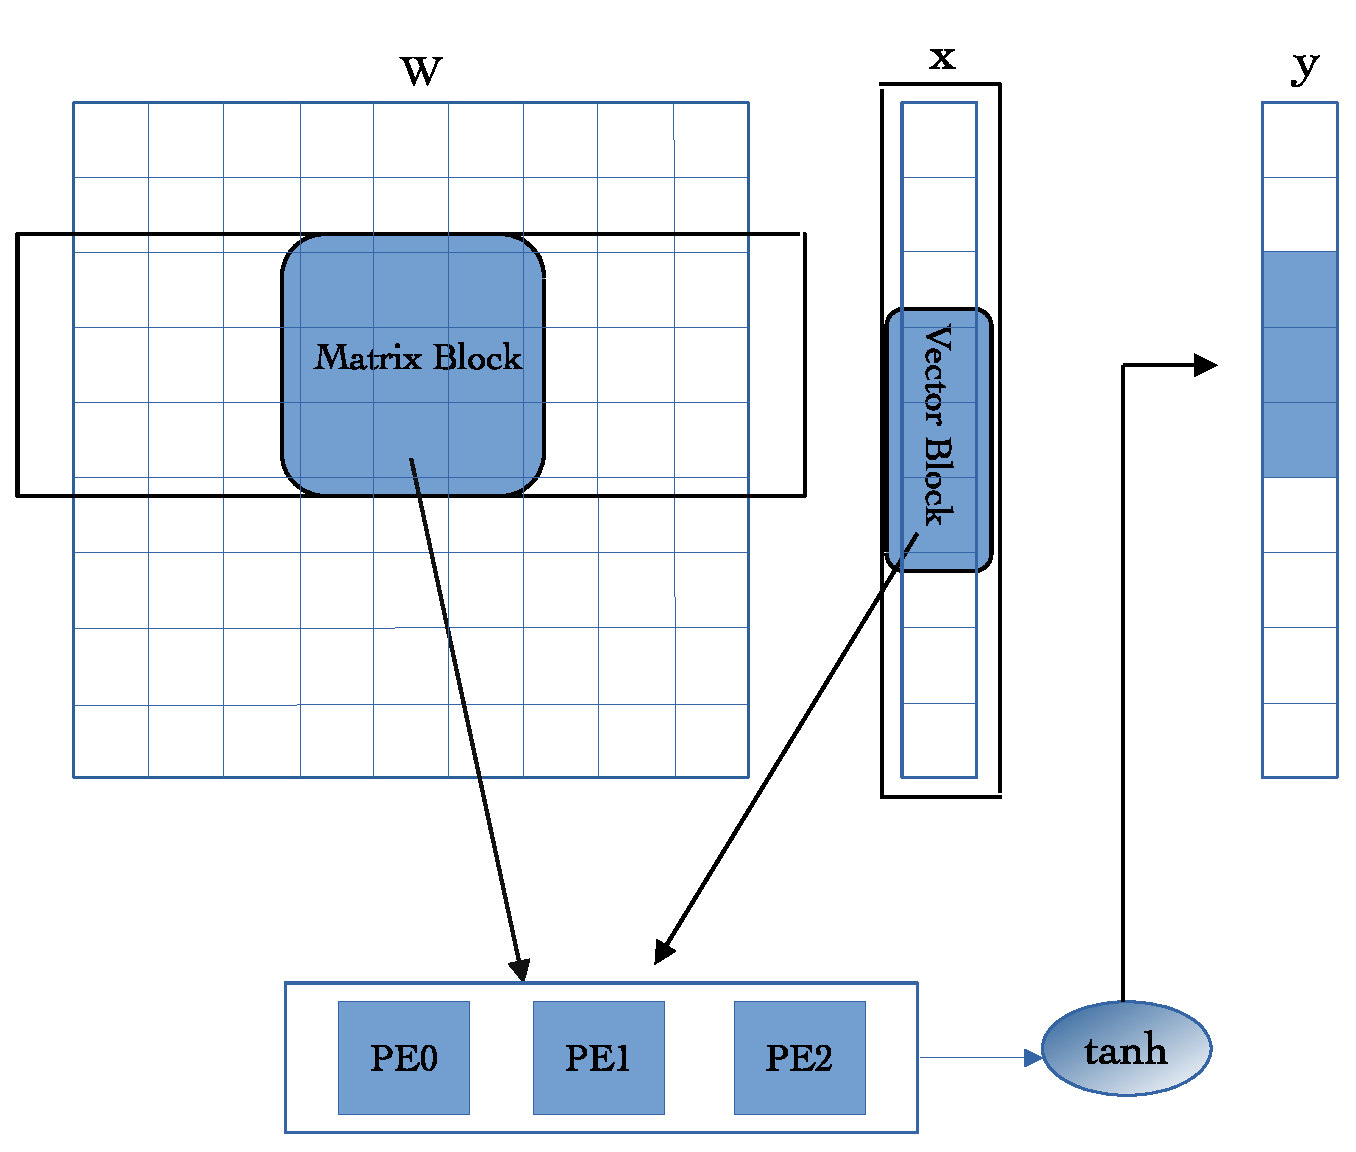
\includegraphics[width=0.6\columnwidth]{exp/fig_compute.eps}
	\caption{计算架构图。基于矩阵向量乘法分块运算的方法设计}
	\label{fig:compute}
\end{figure}
图~\ref{fig:compute} 所示为分块矩阵向量乘法的示意图,图中分块矩阵的大小为\(3 \times 3\),原始矩阵的大小是\(9 \times 9\),因此完成整个矩阵向量乘法
一共需要调用9次分块运算,生成结果向量的单个元素则需要进行3次调用。分块矩阵进行计算时,由于各元素的计算不存在数据依赖,因此可以使用并行
计算的方式,图中将分块矩阵的每一行视为一个独立处理单元(PE),在处理单元的内部还可以使用树形结构以实现进一步的并行。分块矩阵乘法通过
分时复用和内部并行的方式不仅可以计算任意维度的矩阵向量乘法,还能达到加速运算的目的,是满足本文切换网络尺寸需求的一种计算模式。

%介绍分块矩阵乘法,外部可配置,内部可并行


%计算架构的设计目的

%怎么设计:方案1,方案2

%设计结果:

\subsection{存储架构设计}
为了解决存储速度和成本的矛盾,并配合计算架构高效的完成计算任务,本文设计了三级存储系统,如图~\ref{fig:memory} 所示。其中DRAM的存储容量最大,
但是由于其位于片外,远离计算结构,因此存在较大的访存延迟。BRAM是片上同步存储单元,拥有较快的数据移动速度,但是容量较小。寄存器(Register)位于
计算结构的内部,是使用LUT搭建的异步存储单元,响应速度快,是计算结构不可分割的组成部分。

\begin{figure}
	\centering
	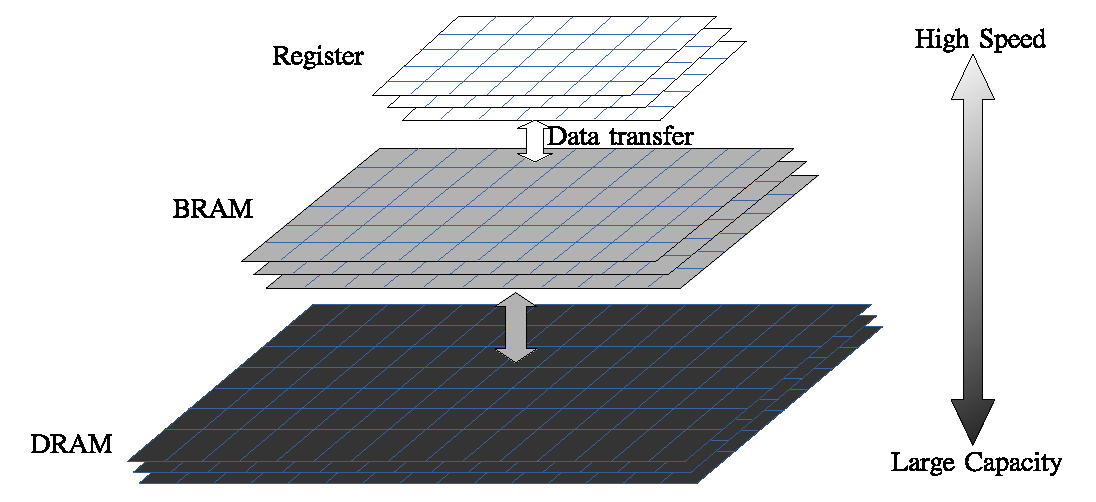
\includegraphics[width=0.7\columnwidth]{exp/fig_memory.eps}
	\caption{存储架构图。“DRAM-BRAM-Register”三级存储系统}
	\label{fig:memory}
\end{figure}

根据存储系统的特性,本文为不同存储结构分配了相应的任务。DRAM用于存储网络模型的权重参数以及必要的压缩信息,这些数据的数量庞大,并且部分数据使用频率
较低。BRAM用于缓存计算结构和DRAM之间交换的数据,在前向传播过程中,一方面其接收来自DRAM中的分块矩阵和向量,另一方面其暂存计算结构的结果,当完成全部数据的计算后,
一次性的将数据迁移到下级存储DRAM中,中间层存储BRAM有效的降低了片上和片外数据的交换次数。寄存器是计算结构的组成部分,用于暂存计算单元的输入,输出和中间计算结果。
数据在经过三级存储系统的传输和缓存后,最终实现了高效的数据处理。
\subsection{激活函数分段近似}

激活函数用于控制神经元之间信息流通的比例,是神经网络中最重要的组成部分。但是硬件电路仅提供基本的数字逻辑,无法直接实现非线性激活函数。
传统上激活函数硬件实现的方法包括查找表法,坐标旋转法,分段近似方法等,不同的方法有不同的实现成本,资源消耗,精度损失和计算延迟,在实际应用过程往往
需要综合考虑以上因素。

本文激活函数的实现首先需要满足高精度的要求,这是因为循环神经网络的循环结构会在不断的累积误差。如果激活函数的误差较大,循环神经网络
将无法准确的完成预测功能。其次,在保证精度的前提下,较低的资源消耗与计算延迟也激活函数高效实现所必需考虑的因素。综合以上设计要求,
本文选用分段近似的激活函数实现方法。
激活函数分段近似的数学表达为式~(\ref{eq:Tanh_approx})
\begin{equation}
f(x) = 
  \begin{cases} 
  \quad 1			&  x \geq L \\
  \quad H(x)     	&  -L < x < L	\\
  \quad -1			& 	x\leq -L
  \end{cases}
\label{eq:Tanh_approx}
\end{equation}
其中L表示近似边界,当\(x\)超过边界时,认为激活函数已经饱和。\(H(x)\)是近似函数,不同的近似方法有不同的函数形式。本文采用三次函数的近似方法,
其函数形式为
\begin{equation}
H(x) = ax^3 + bx^2 + cx +d	\\
\end{equation}
函数近似难免会存在精度损失,因此为了进一步提高精度,激活函数的非饱和区间\([-L,L]\)将会继续被分段,在每个分段区间上都会采用三次函数进行拟合
并获得三次拟合的系数。分段点数量越多,分段近似函数的精度越高,但是考虑到硬件实现的资源消耗,分段点越少资源消耗越低。具体分段的数量需要根据
任务的精度要求和数值范围进行确定,例如本文的分段数量为10,采用均匀分段的方法,均方误差为\(4.21 \times 10^{-6}\)。
\begin{figure}[htbp]
	\centering
		\subfloat[]{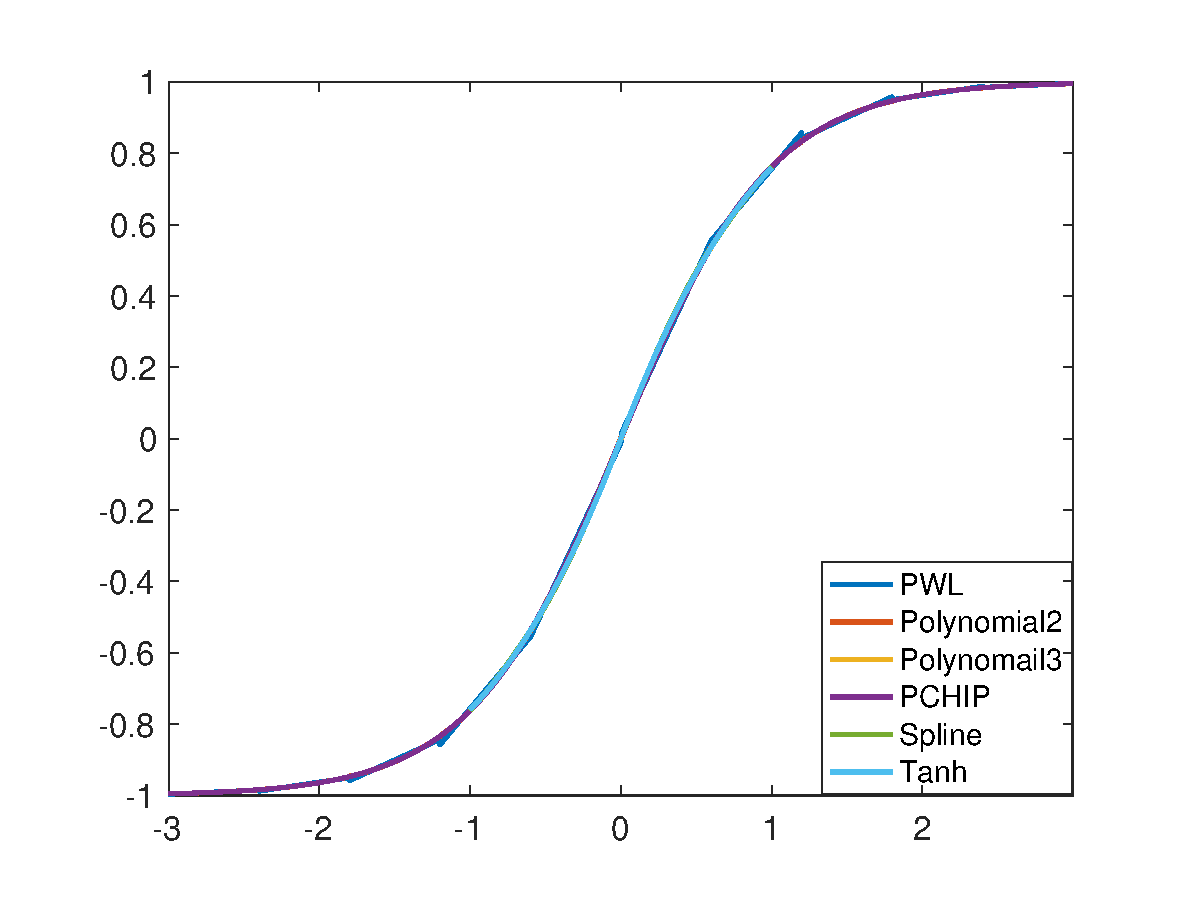
\includegraphics[width=0.45\linewidth]{exp/fig_activation33.eps}}
		\subfloat[]{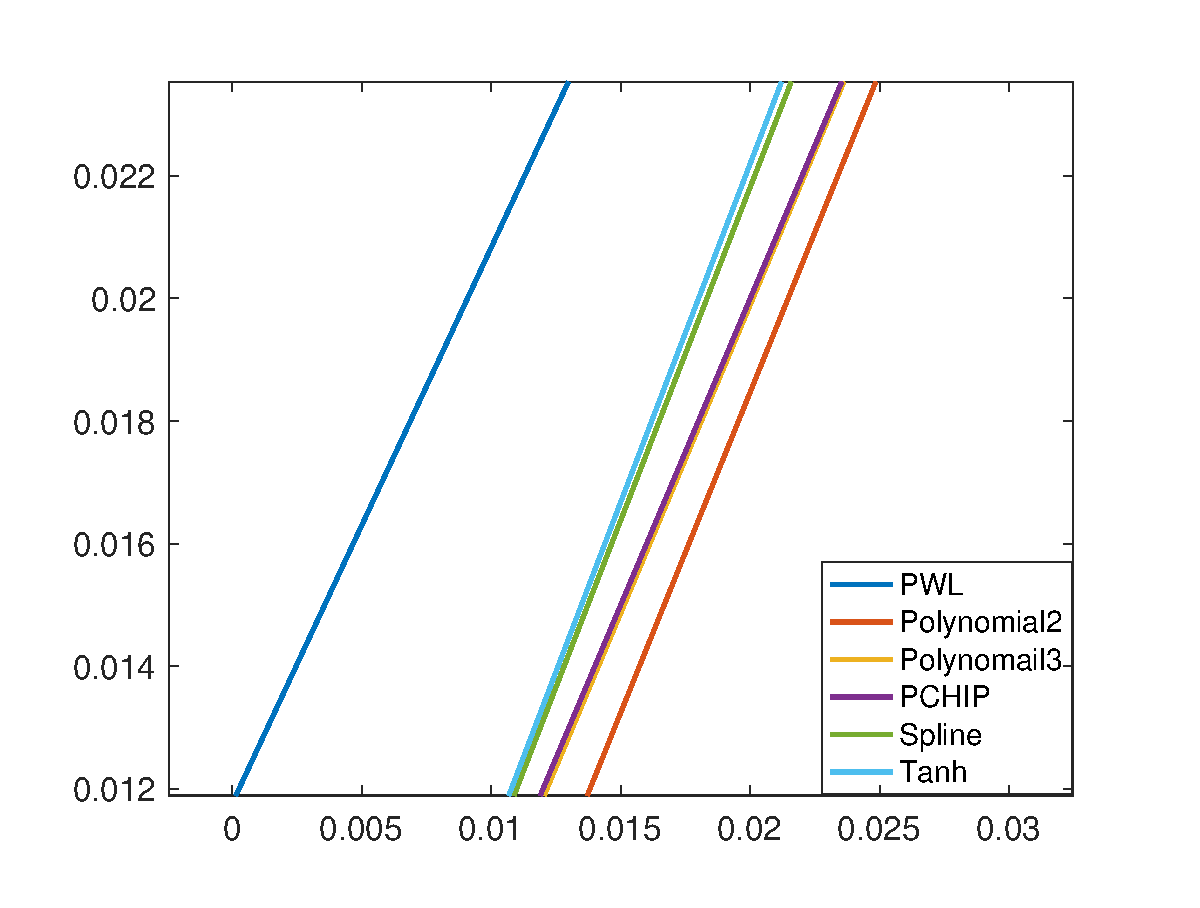
\includegraphics[width=0.45\linewidth]{exp/fig_activation33_zoom.eps}}	
	\caption{不同分段近似方法的激活函数近似效果,图a是在区间[-3,3]的整体效果,图b是在0附近的局部放大效果}
\label{fig:activationErr}
\end{figure}

%为了便于硬件实现,提取函数中的基本操作单元,三次近似函数可进一步表示为

图~\ref{fig:activationErr} 展示了不同分段近似方法的激活函数近似效果。整体而言,所有的近似方法都能较好的贴合激活函数,不同的近似方法存在
微小的精度差异,如图b所示,其中线性近似方法误差较大,其余的非线性近似方法误差较小。表~\ref{tab:activation} 展示了不同近似方法的误差值,其中PCHIP,
Splines 3和三次多项式近似据均有较小的误差,并且都能满足任务的精度需求,考虑到这三种方法的硬件结构相同,因此本文最终选用精度较高的三次多项式近似的方法。
实际上,无论线性近似,二次函数近似还是三次函数近似,在硬件实现时都有相似的基本结构,提取函数的基本操作单元,三次函数可进一步表示为
\begin{equation}
H(x) = x(x(ax+b)+c) + d
\end{equation}
式中\(ax+b\)即为近似方法通用的基本操作单元。

\begin{center}
\begin{table}
	\caption{激活函数不同分段近似方法及其误差}
	\renewcommand\arraystretch{1.2}
	\setlength{\tabcolsep}{60pt}
	\begin{tabular}{cc}
		\toprule
		Approximation			&				RMSE		\\	\midrule
		PWL						&				4.30 \(\times 10^{-2}\)		 	\\	
		Polynomial D.2			&				1.13 \(\times 10^{-4}\)			\\
		Polynomial D.3			&				4.21 \(\times 10^{-6}\)			\\
		PCHIP					&				3.22 \(\times 10^{-4}\)			\\
		Splines 3				&				5.59 \(\times 10^{-5}\)			\\
	\bottomrule
	\label{tab:accuracy}
	\end{tabular}
\end{table}
\end{center}

\vspace{-4em}
\section{硬件加速器的实现}
%\subsection{控制单元设计}

\subsection{矩阵向量乘法模块}
矩阵向量乘法的基本处理单元是PE,其完成的功能是对两个相同维度的向量进行内积操作,通过堆叠PE形成计算单元(CU)可以实现小规模
的矩阵向量乘法,即本文中的分块矩阵向量乘法。PE的基本结构如图~\ref{fig:MVM} 所示,其中图(a)展示了向量乘法的循环累积实现形式,该实现方式消耗的
计算资源仅为一个乘法器和一个加法器。对于n维向量的乘法,需要执行n次乘法和n-1次加法操作,时间为\(\mathcal{O}(2n-1)\)。图(b)展示了向量乘法的树形实现方式,
该实现方式通过并行乘法和加法运算,时间复杂度降低为\(\mathcal{O}(log(n))\)。树形结构的大小取决于运算资源的数量以及任务的实际需求,在本文的设计中
PE的维度是10。更大的并行度会带来更大的加速能力,但也可能导致更多的性能浪费,尤其是当矩阵向量的维度低于PE的维度时,部分乘法器和加法器
处于空转的状态。为了解决这一问题,本文采用了较低的PE维度,但在CU层面使用了更多并行的PE单元并形成阵列,这种紧凑的计算结构使得计算
资源被充分利用,效率更高。图~\ref{fig:MVM_long} 所示为高维PE和低维PE并行结构的示意图,其中颜色越深,表示利用率越高,明显的,
紧凑的低维PE结构拥有更高的利用率。
\begin{figure}[htbp]
	\centering
		\subfloat[]{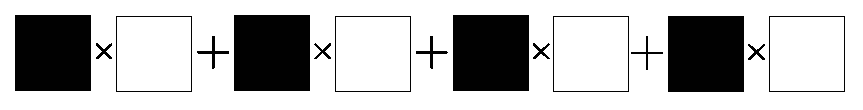
\includegraphics[width=0.37\linewidth]{exp/fig_MVM_element.eps}}	\\
		\subfloat[]{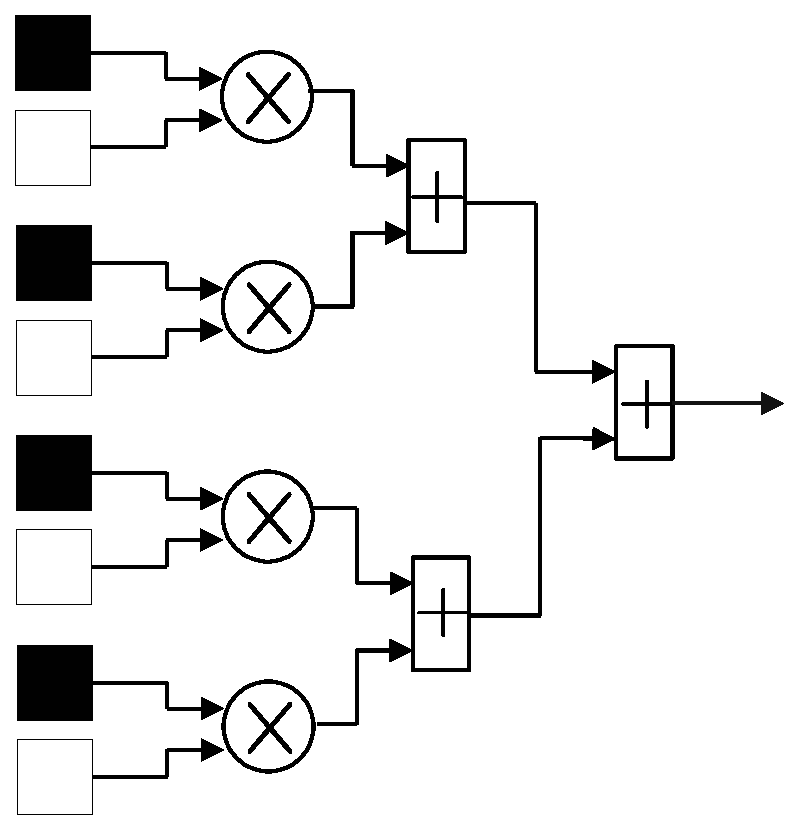
\includegraphics[width=0.35\linewidth]{exp/fig_MVM.eps}}	
	\caption{(a)向量乘法的循环累积方式,(b)向量乘法的树形累积形式}
\label{fig:MVM}
\end{figure}
\begin{figure}[htbp]
	\centering
		\subfloat[]{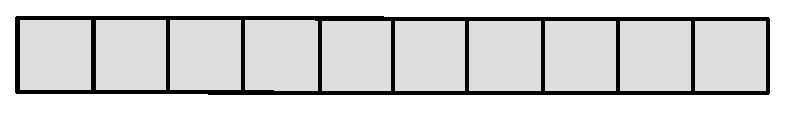
\includegraphics[width=0.37\linewidth]{exp/fig_MVM_long.eps}}	\\
		\subfloat[]{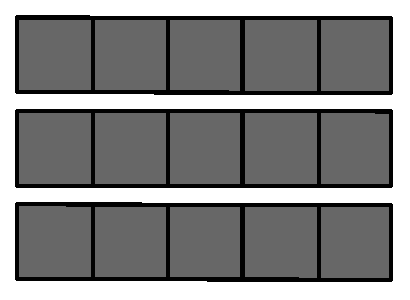
\includegraphics[width=0.20\linewidth]{exp/fig_MVM_short.eps}}	
	\caption{(a)高维PE计算单元,(b)多个低维PE计算单元组成CU结构}
\label{fig:MVM_long}
\end{figure}


\subsection{激活函数模块}
本文使用分段三次函数近似的方法实现激活函数,其硬件结构如图~\ref{fig:tanh} 所示。首先输入会经过输入预处理单元,该硬件单元会将输入转化为分段区间地址用以索引近似函数的相关系数,
其中具体包括绝对值运算和地址偏移运算。然后输入的绝对值\(|x|\)和三次函数的系数(\(a,b,c,d\))将会被送到非线性函数运算单元,在经过三个时钟周期的乘加运算后,该单元会输出近似的激活函数值。
最后,输出单元将输入的符号位添加到激活函数的输出值上作为激活函数的最终输出。以上详细说明了激活函数模块数据处理的流程,其大致可以划分为分段和计算两大步骤。实际上,该流程也适用于
其他分段近似激活函数的硬件实现,仅需要调整非线性函数运算单元的计算周期就能实现不同次数多项式的近似。
\begin{figure}[htbp]
	\centering
	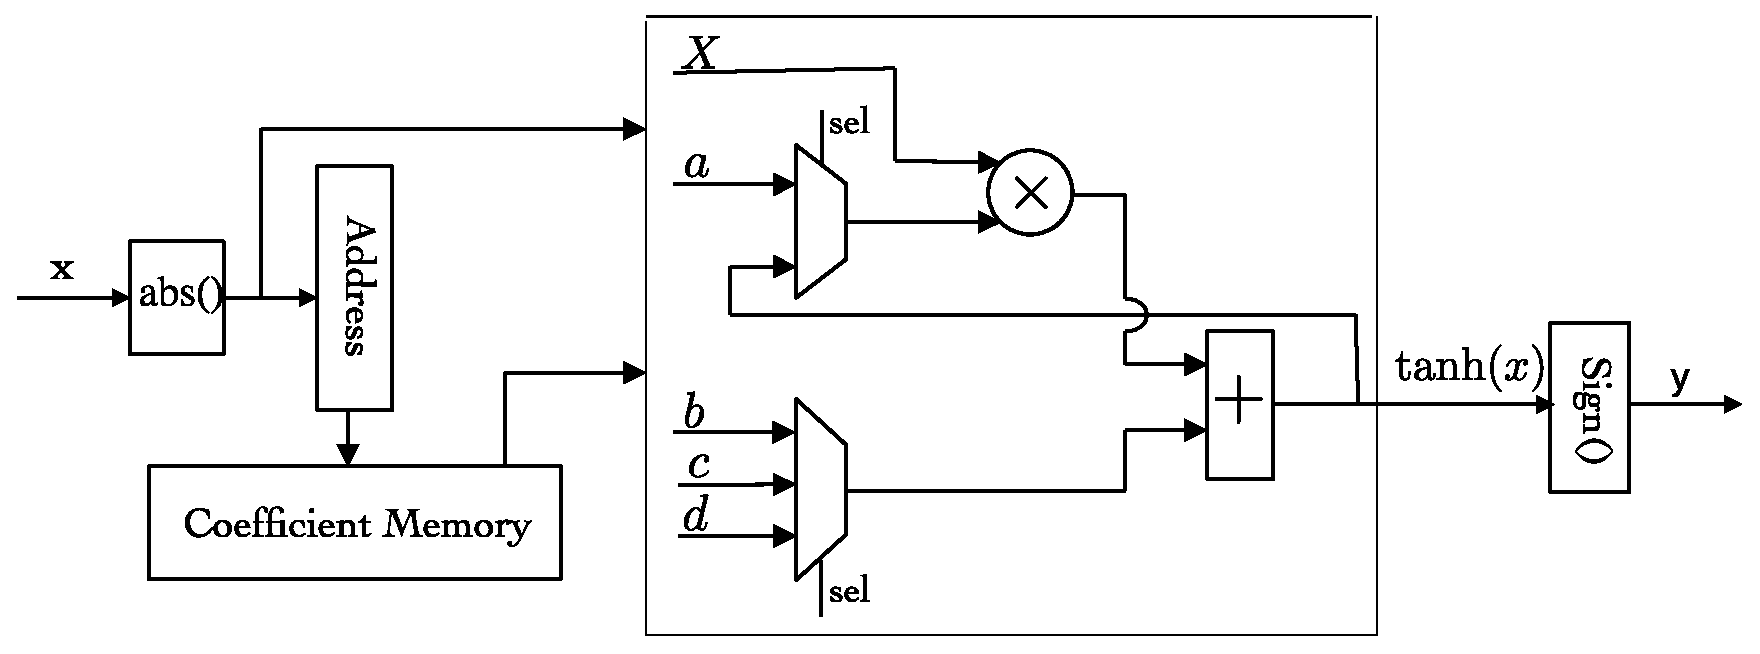
\includegraphics[width=1\columnwidth]{exp/fig_activation_hard.eps}
	\caption{激活函数硬件结构图}
	\label{fig:tanh}
\end{figure}
\subsection{IP核互联设计}
\begin{figure}[htbp]
	\centering
	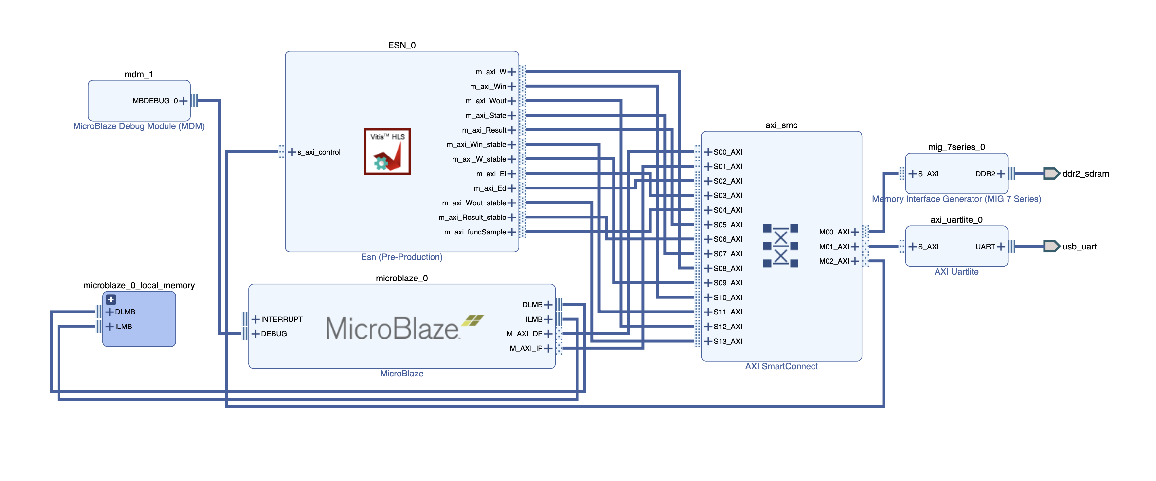
\includegraphics[width=1\columnwidth]{exp/fig_blockDesign.eps}
	\caption{IP核互连示意图}
	\label{fig:blockDesign}
\end{figure}
图~\ref{fig:blockDesign} 展示了系统主要IP模块及其互联,其中包括ESN加速器模块,Mciroblaze软核模块,片外存储DDR模块,以及Uart通信模块。
系统中的各模块通过AXI总线相互连接,实现数据的交换以及任务的分工协作。ESN加速器模块负责实现系统最主要的功能---网络的前向传播,该功能的实现
需要依赖系统其他IP模块的配合,具体流程如下:首先,软件端通过Microblaze核配置加速器的各参数地址信息,并传输启动的命令。然后,加速器通过其内部的DMA
模块将数据从指定的地址搬运到片上存储单元,计算单元在获取这些数据后将会执行网络的前向传播计算功能。最后在完成计算后,加速器会将结果返回到软件端。
其他的功能如模型压缩等,也是在软件端的控制下,将功能映射到具体的硬件模块进行执行。


\section{本章小结}
本章围绕循环神经网络加速技术的具体实现,详细地分析并讨论了包括算法,软件,硬件以及系统集成等方面的技术。首先,在章节的开始部分,本章
详细的分析了简化循环神经网络的结构特性,然后就如何获得这样这样一个简化网络模型展开了详细的介绍,给出了网络压缩算法的具体推导过程,包括状态近似和
激活函数近似。然后通过分析压缩算法的特性发现其具有压缩成本低,无需数据集,精度损失小等优势。结合实际应用需求与算力支持,压缩算法和网络的前向传播
可以组成独立完整的系统,该系统能够满足用户和环境对速度和精度的弹性需求,具有很大的应用价值和广阔的前景。因此,系统的设计与实现是本章后续讨论的重点,
并且也是本文的主要任务。在分析系统的运行流程并进行合理的软硬件功能划分后,本章提出了系统整体架构。在软件实现方面,本章给出了软件主要功能的算法,并提出了基于采状态采样的模型生成方法和基于预存投影矩阵的模型生成方法;
在硬件实现方面,本章详细分析了网络前向传播算法的加速空间,并提出了满足系统需求的硬件加速器结构。最后本章详细的介绍了加速器的具体实现过程,
包括架构层面的设计:计算架构设计和存储架构设计,也包括硬件模块的具体实现:矩阵向量乘法模型和激活函数模块。在完成以上具体功能部件的设计后,
本章基于FPGA搭建了系统。
